% KOMA-Script scrbook template for XeLaTeX
% Encoding: UTF-8
% Usage:
%   xelatex -interaction=nonstopmode -halt-on-error komascript_book_xelatex.tex
% Or use pandoc: pandoc src/book/chapter1.md --template=latex/komascript_book_xelatex.tex -o output/book.tex
\documentclass[fontsize=12pt, paper=a4, oneside, openany]{scrbook}

% XeLaTeX and CJK
\usepackage{fontspec}
\usepackage{xeCJK}
\usepackage{microtype}
\usepackage{graphicx}
\usepackage{hyperref}
\usepackage{bookmark}
\usepackage{longtable}
\usepackage{amsmath,amssymb}
\usepackage{listings}
\usepackage{geometry}
\usepackage{caption}
\usepackage{titling}

% Page geometry
\geometry{a4paper, left=28mm, right=28mm, top=30mm, bottom=30mm}

% Fonts (adjust if you have other preferred fonts)
% \setmainfont{Noto Serif}
% \setsansfont{Noto Sans}
% \setmonofont{Source Code Pro}
\xeCJKsetup{CJKmath=true}
% \setCJKmainfont{Noto Sans CJK SC}

% Hyperref setup
\hypersetup{
    colorlinks=true,
    linkcolor=blue,
    citecolor=blue,
    urlcolor=blue,
    pdftitle={Ascend310 Book},
    pdfauthor={周贤中}
}

% KOMA options
\KOMAoptions{chapterprefix=true, headings=big}
\setkomafont{disposition}{\normalfont\bfseries}

% Header/Footer
\usepackage{fancyhdr}
\pagestyle{fancy}
\fancyhf{}
\fancyhead[LE,RO]{\thepage}
\fancyhead[LO]{\leftmark}
\fancyhead[RE]{\rightmark}
\renewcommand{\headrulewidth}{0.4pt}
\renewcommand{\footrulewidth}{0pt}

% Title
\title{Ascend310 实战手册}
\author{周贤中}
\date{\today}

% Pandoc: allow metadata variables
% pandoc will replace variables like $title$, $author$ if provided
\providecommand{\booktitle}{$if(title)$$title$$else$Ascend310 实战手册$endif$}

\begin{document}
\frontmatter
\maketitle
\tableofcontents
\mainmatter

% Include body (pandoc can replace) or input a single compiled file
% \hypertarget{ux6607ux817e310bux5f00ux53d1ux677fux4ecbux7ecd}{%
\section{昇腾310B开发板介绍}\label{ux6607ux817e310bux5f00ux53d1ux677fux4ecbux7ecd}}

OrangePi
AIpro(8T)开发板是香橙派联合华为精心打造的高性能AI开发板,采用昇腾AI技术路线,搭载的昇腾310B为4核64位处理器+AI处理器,集成图形处理器,支持8TOPS
INT8的AI算力,拥有8GB/16GB LPDDR4X内存,可以外接32GB/64GB/128GB/256GB
eMMC模块,支持双4K高清输出。OrangePi
AIpro(8T)引用了相当丰富的接口,包括两个HDMI输出、GPIO接口、Type-C电源接口、支持SATA/NVMe
SSD 2280的M.2插槽、TF插槽、千兆网口、两个USB3.0、一个USB Type-C
3.0、一个Micro
USB(串口打印调试功能)、两个MIPI摄像头、一个MIPI屏等,预留电池接口,可广泛适用于AI边缘计算、深度视觉学习及视频流AI分析、视频图像分析、自然语言处理、智能小车、机械臂、人工智能、无人机、云计算、AR/VR、智能安防、智能家居等领域,覆盖
AIoT各个行业。 OrangePi
AIpro(8T)支持Ubuntu、openEuler操作系统,满足大多数AI算法原型验证、推理应用开发的需求。
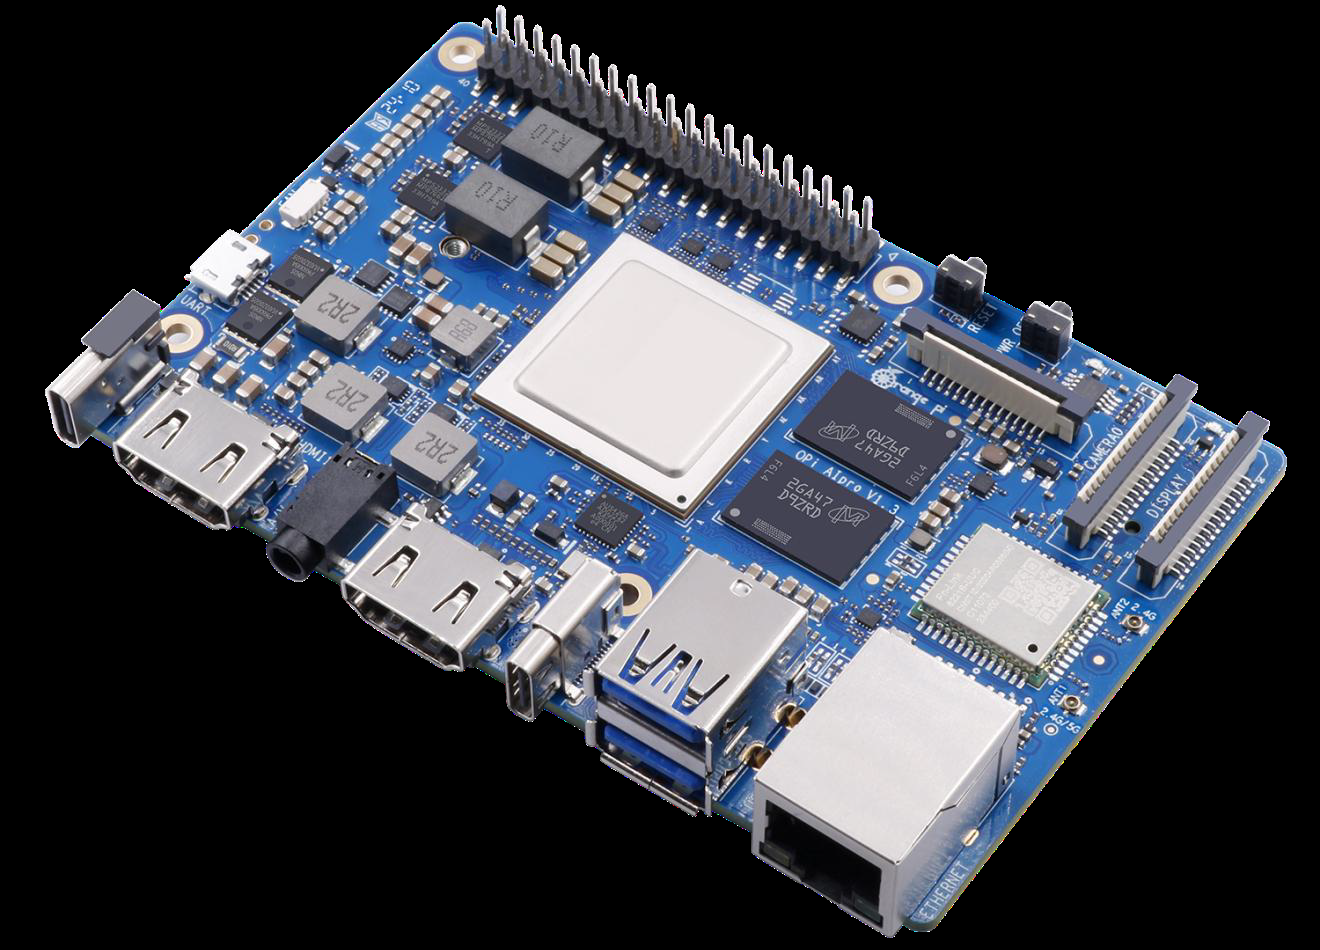
\includegraphics{img0/aipro.png}

\hypertarget{ux5f00ux53d1ux677fux8be6ux7ec6ux89c6ux56fe}{%
\subsection{开发板详细视图}\label{ux5f00ux53d1ux677fux8be6ux7ec6ux89c6ux56fe}}

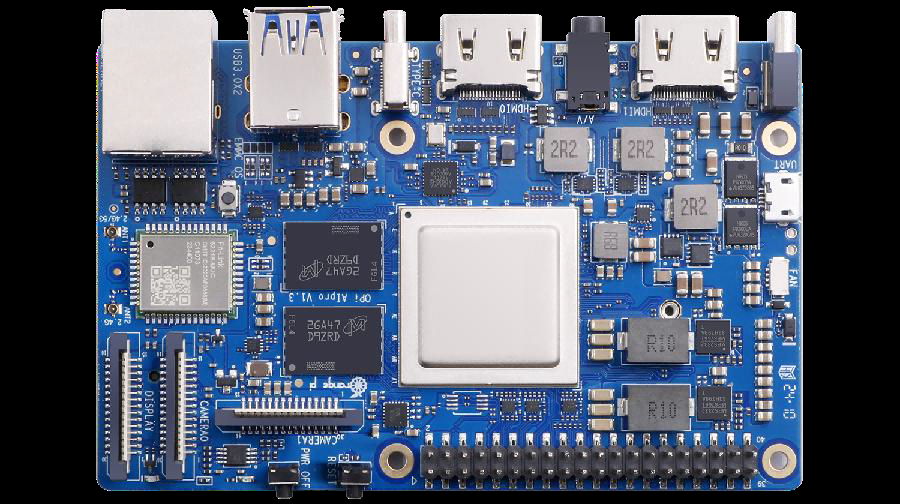
\includegraphics{img0/4.png} 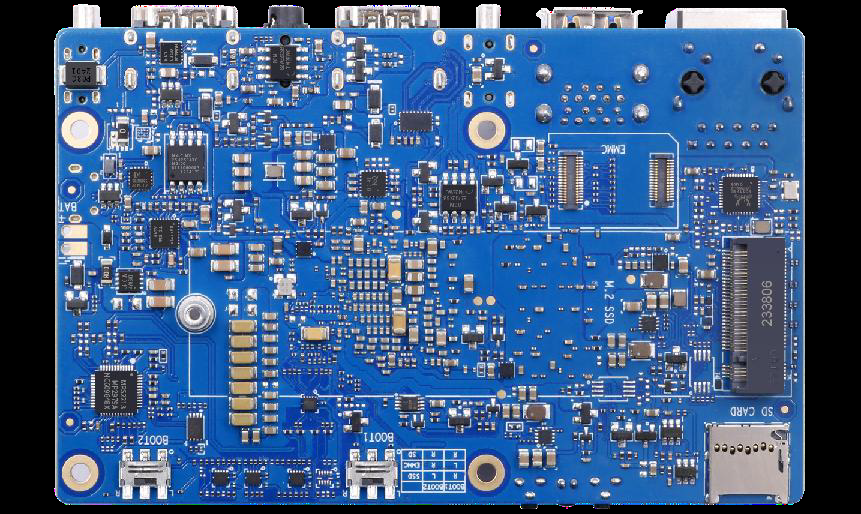
\includegraphics{img0/5.png}
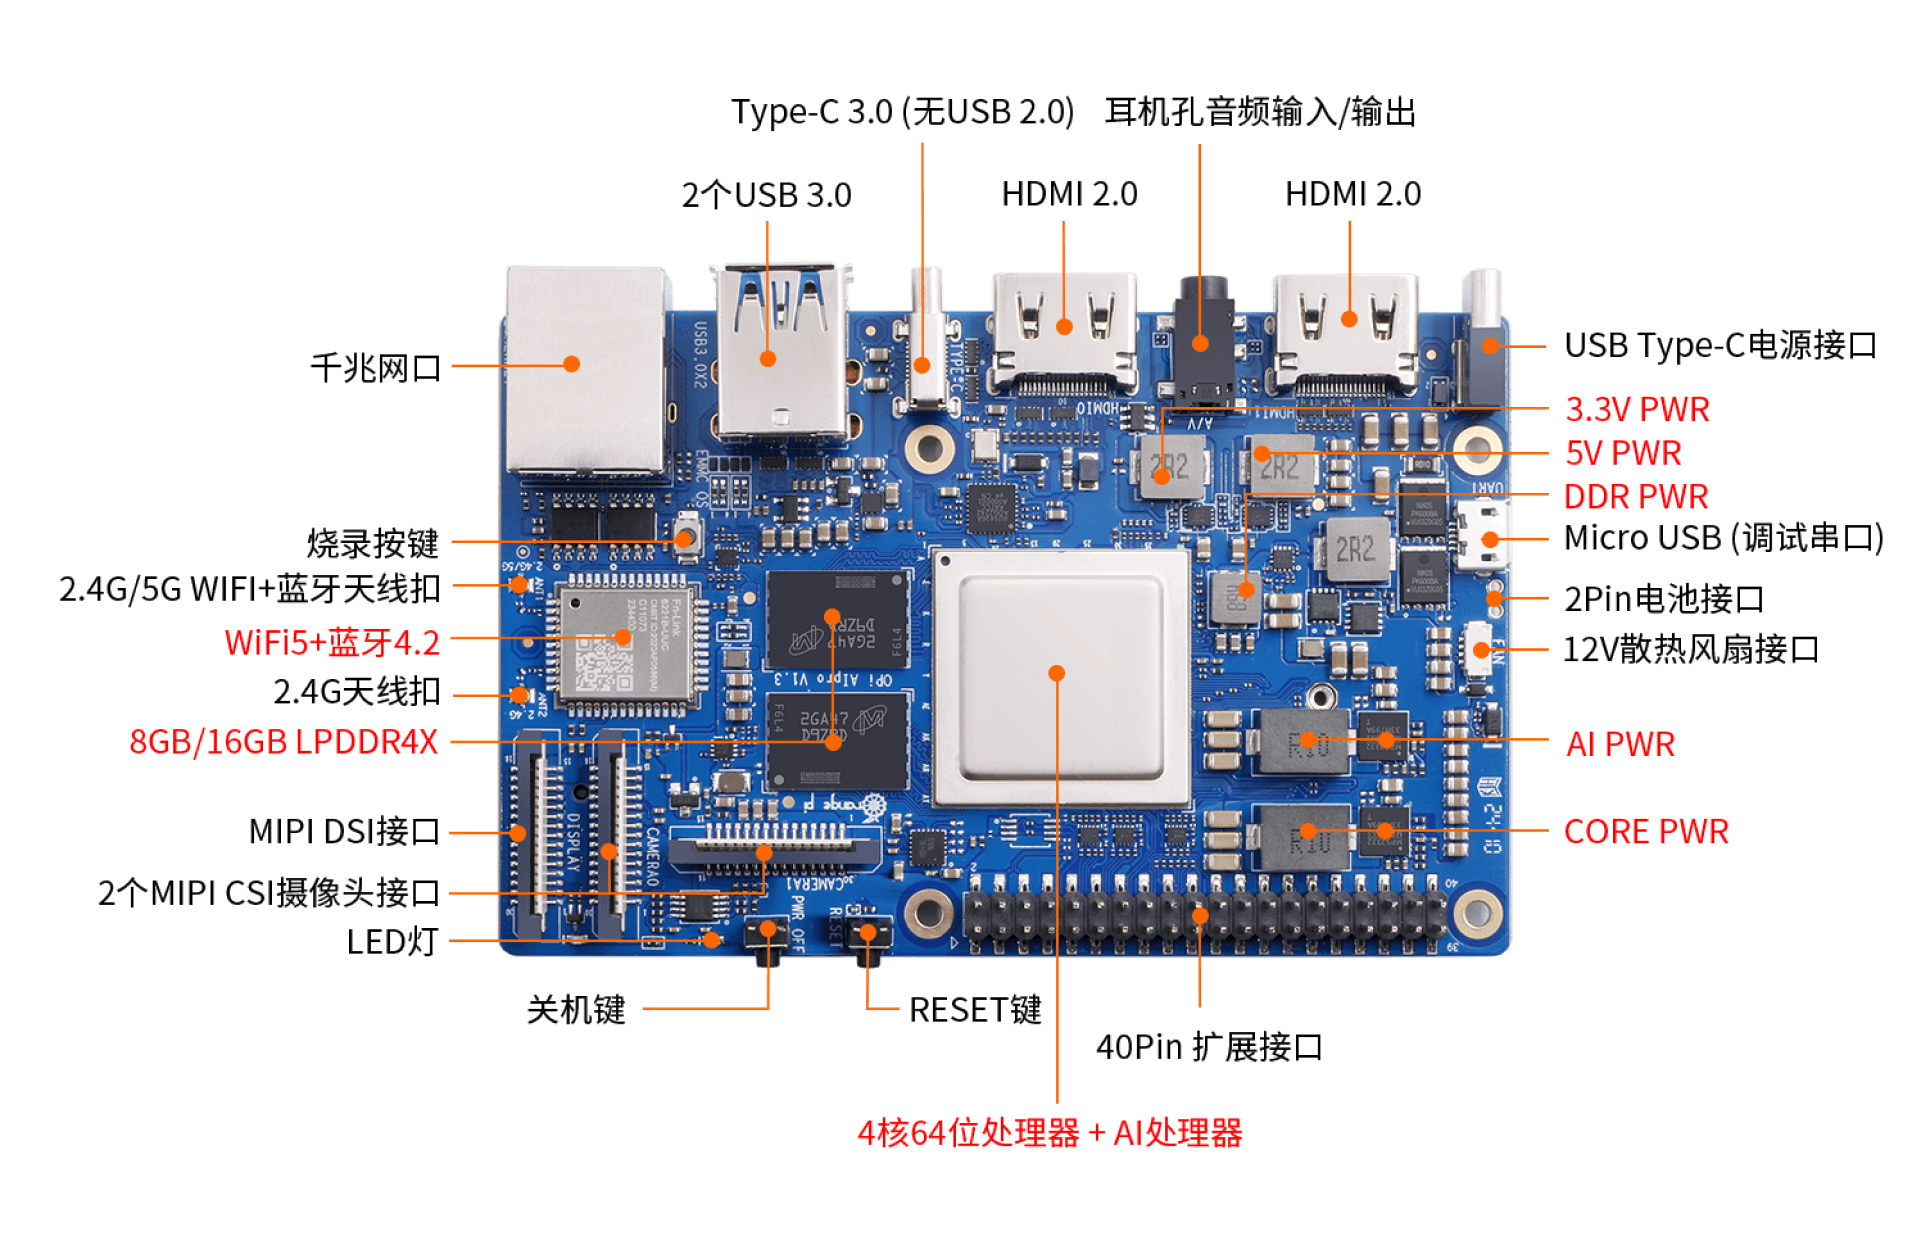
\includegraphics{img0/1.png} 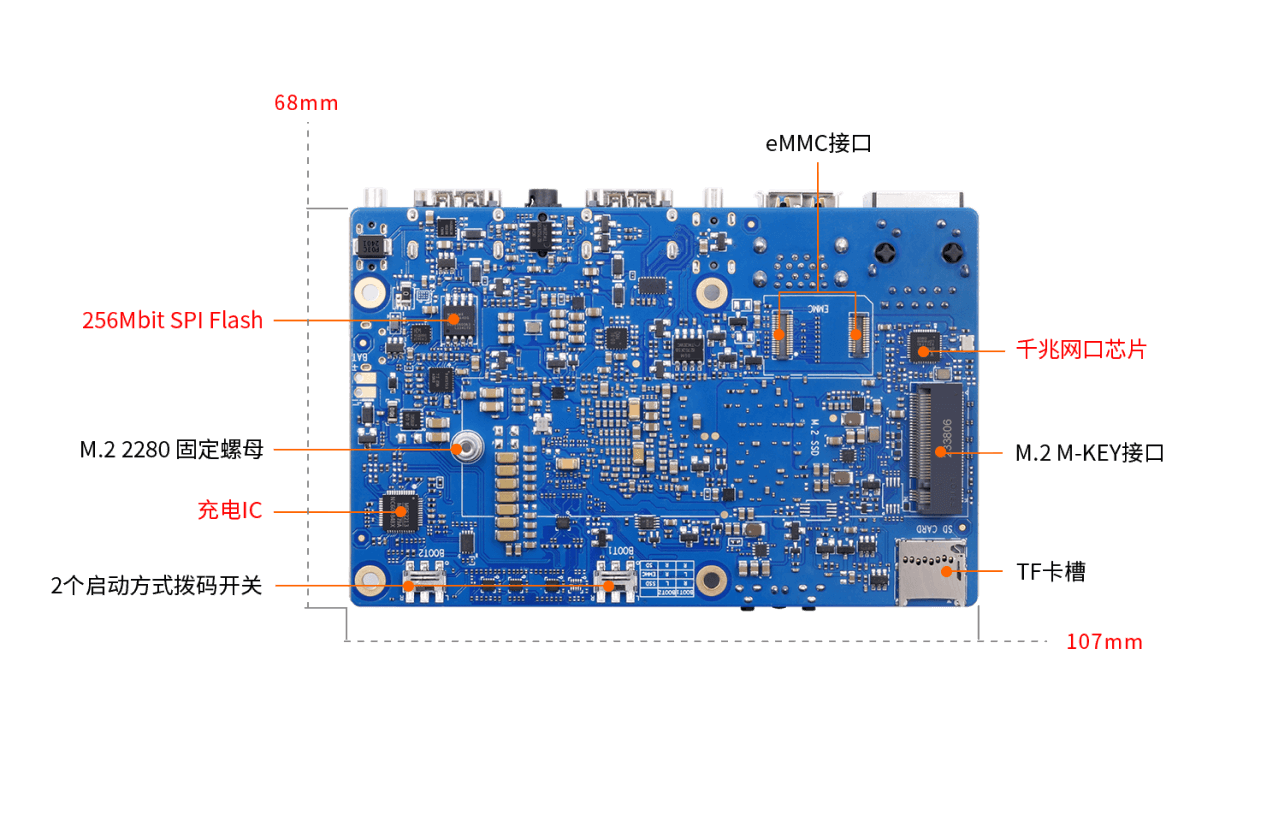
\includegraphics{img0/2.png}
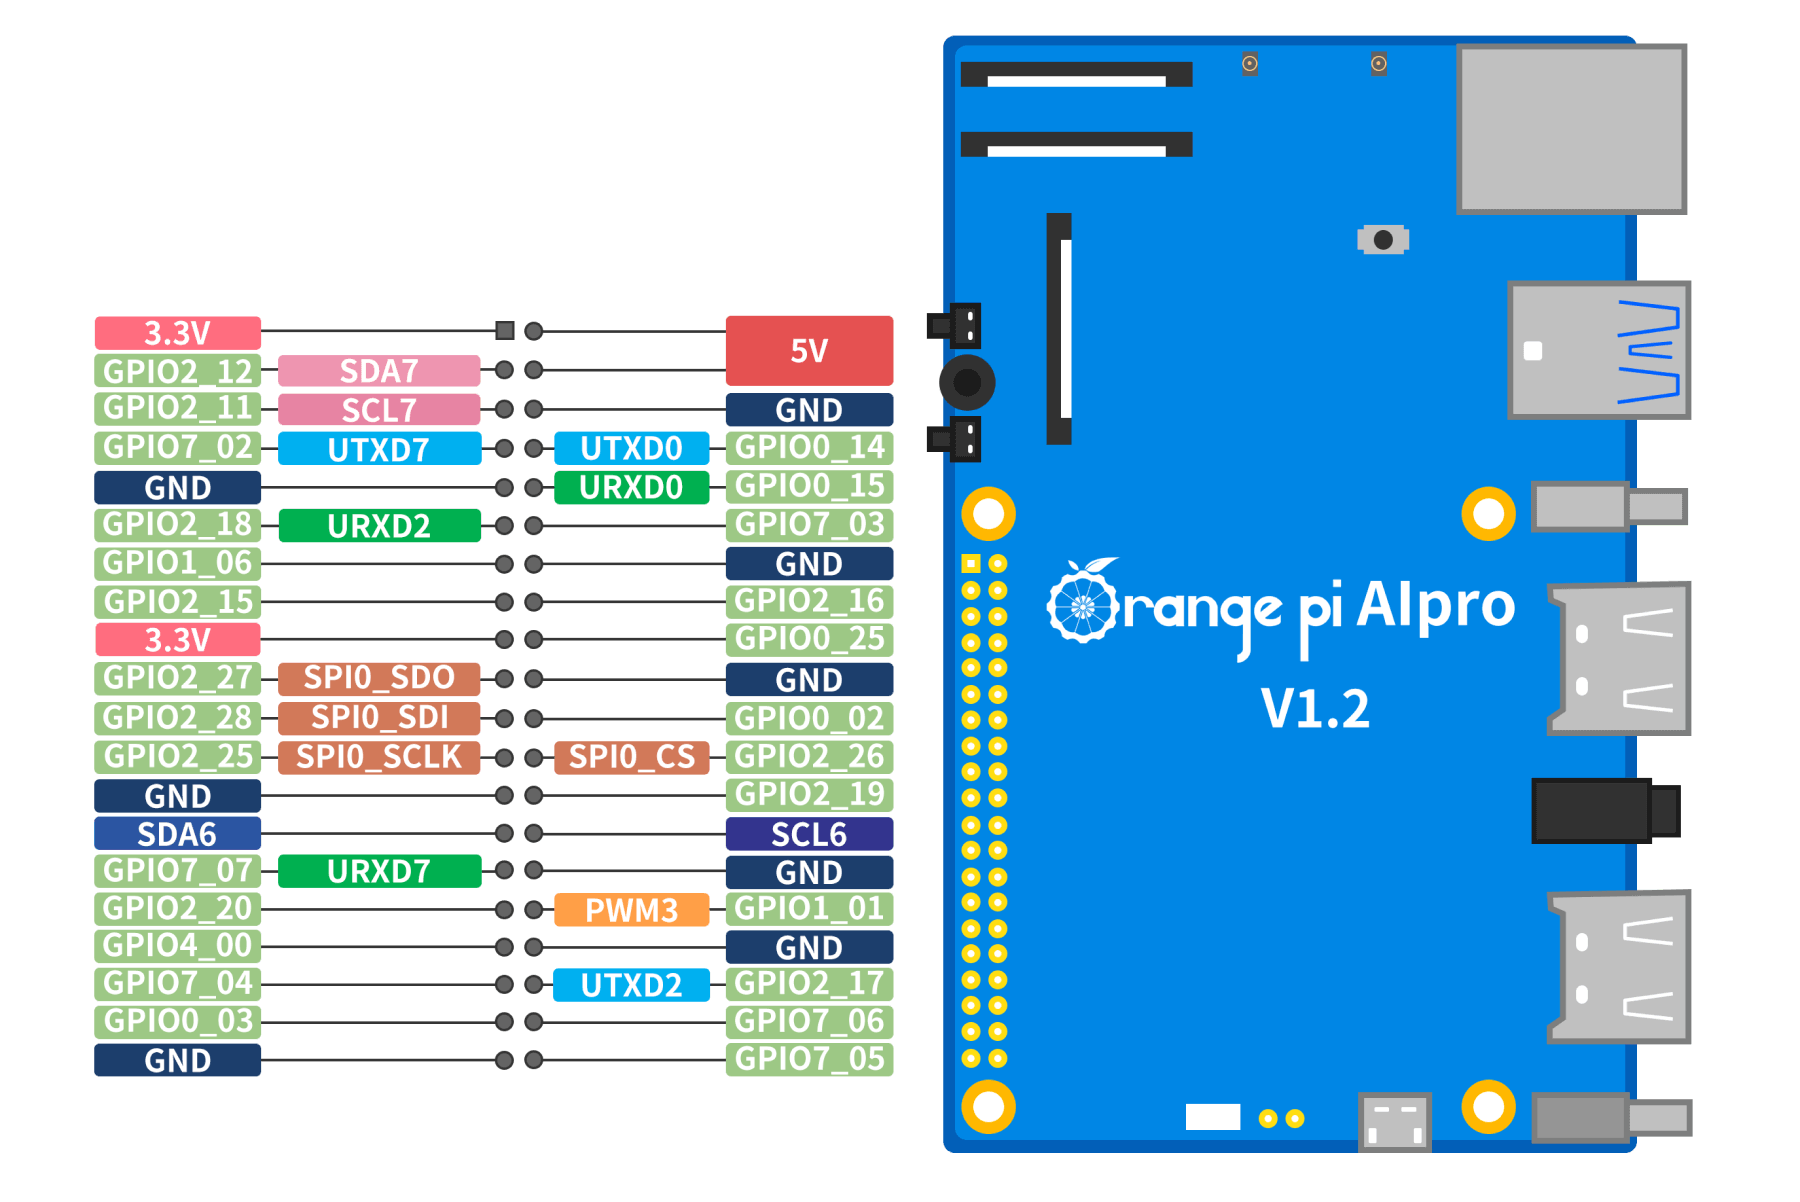
\includegraphics{img0/3.png}

\hypertarget{ux5f00ux53d1ux677fux786cux4ef6ux89c4ux683c}{%
\subsection{开发板硬件规格}\label{ux5f00ux53d1ux677fux786cux4ef6ux89c4ux683c}}

\begin{center}\rule{0.5\linewidth}{0.5pt}\end{center}

\hypertarget{ux6240ux9700ux914dux4ef6}{%
\subsection{所需配件}\label{ux6240ux9700ux914dux4ef6}}

\begin{enumerate}
\def\labelenumi{\arabic{enumi}.}
\item
  TF卡
  容量最小为32GB,速率为Class10级以上的闪迪品牌的TF卡,如下图所示。建议使用64G及以上的TF卡,以避免在开发过程中出现磁盘空间不足的问题。
  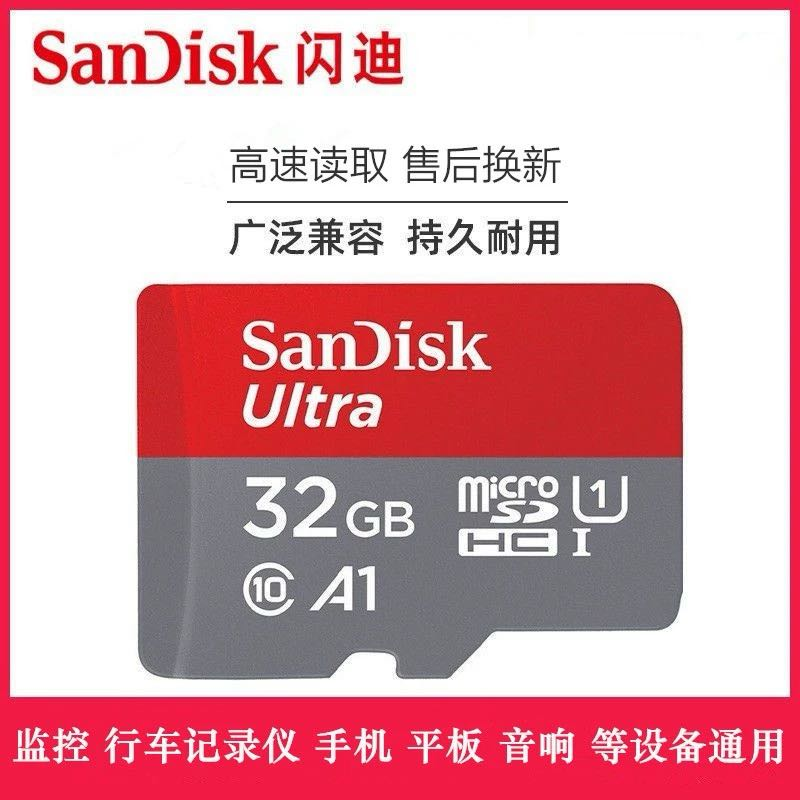
\includegraphics{img1/tf.jpg}
\item
  TF卡读卡器
  用于读写TF卡,刷写系统,建议选择速率为USB3.0以上的,减少系统刷写的等待时间。
  
\includegraphics{img1/reader.jpg}
\item
  HDMI线或HDMI转mini-HDMI线
  主要取决于显示器的接口类型该开发板的视频输出接口为标准HDMI接口。
  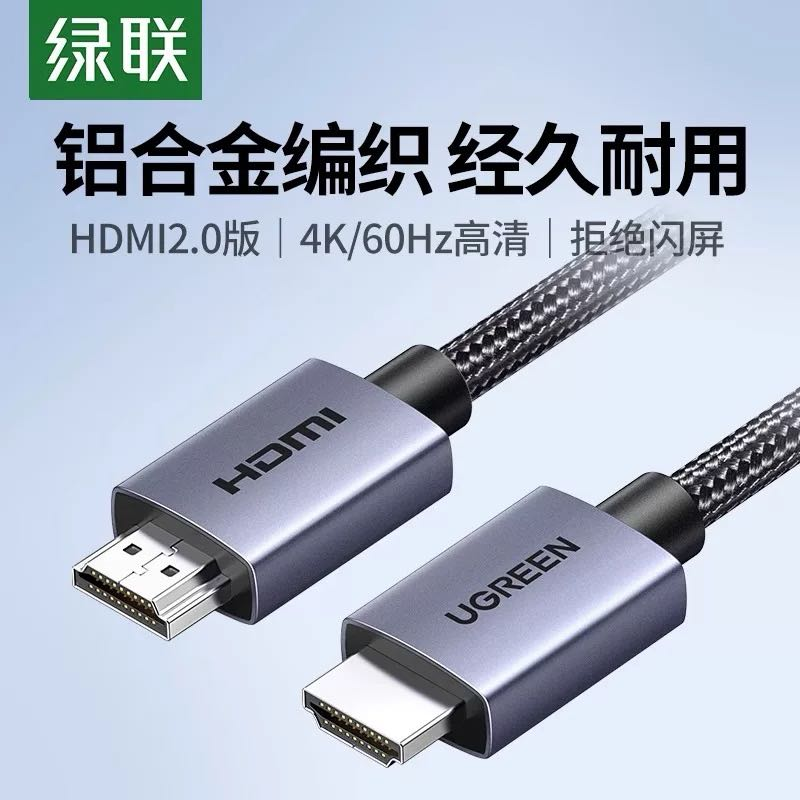
\includegraphics{img1/hdmi.jpg} 
\includegraphics{img1/minihdmi.jpg}
\item
  电源 该开发板的电源输入为PD
  20V,需要搭配支持PD协议20V挡位的65W电源适配器。
  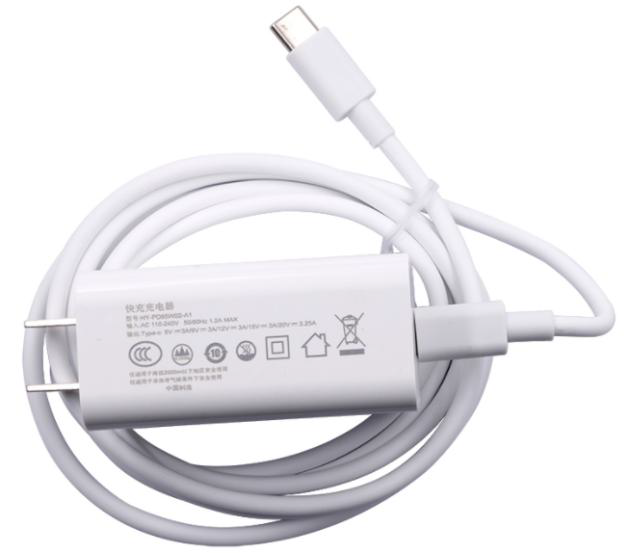
\includegraphics{img1/power.png}
\item
  USB接口的鼠标以及键盘 在无远程访问的条件下对开发板进行本地调试。
  
\includegraphics{img1/mouse.png}
\item
  金属配套外壳 用于保护开发板硬件。 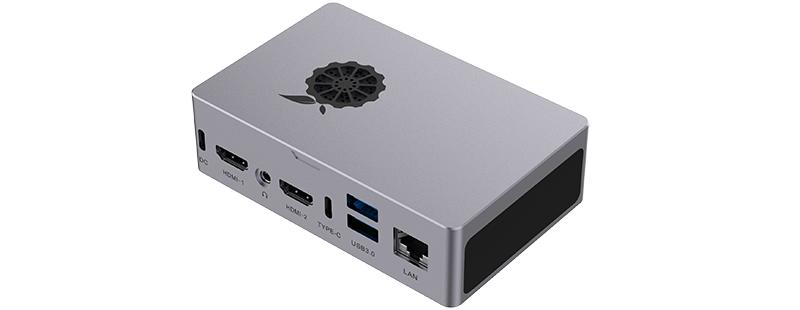
\includegraphics{img1/cover.png}
\item
  12V散热风扇以及散热鳍块
  开发板的风扇接口为2pin,输出电压为12v,支持PWM调速。由于该开发板的CPU发热较大,强烈建议安装主动扇热设备。
  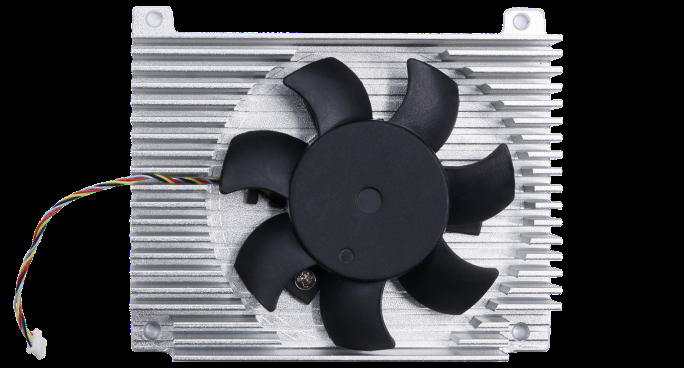
\includegraphics{img1/fan.png}
\item
  Type-C转USB 3.0转接线(可选) OrangePi
  AIPro开发板具有一个Type-C接口,协议为USB3.0(不支持USB
  2.0),可外接支持USB3.0以上协议的外置设备。
  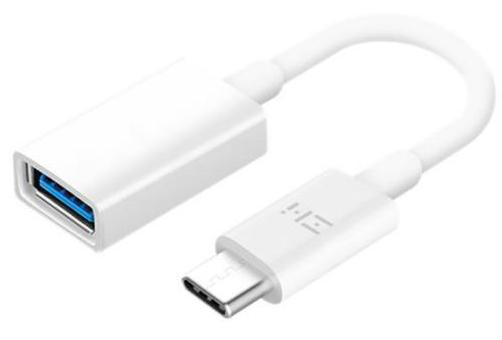
\includegraphics{img1/otg.png}
\item
  M.2接口 2280规格的PCIe Nvme SSD(可选)
  开发板的背部设计有M.2接口,可外接一个M.2的SSD作为开发板的系统盘或者存储。
  
\includegraphics{img1/nvme.png}
\item
  M.2接口 2280规格的Sata Ngff SSD(可选)
  同样,开发板的M.2接口不仅支持PCIe协议,也支持Sata协议,因此也可以使用Sata协议的SSD。
  
\includegraphics{img1/ngff.png}
\item
  香橙派的eMMC模块(可选)
  eMMC(嵌入式多媒体卡)是一种集成了闪存和控制器的低成本存储解决方案,主要用于智能手机、平板电脑和低端笔记本电脑等消费电子产品。其读写速度适中(100-400MB/s),比传统机械硬盘快但不及固态硬盘(SSD),具有体积小、功耗低和易于集成的特点。开发板支持使用eMMC模块作为存储,但需要额外购置eMMC模块。
  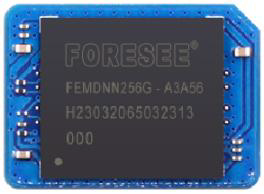
\includegraphics{img1/emmc1.png} 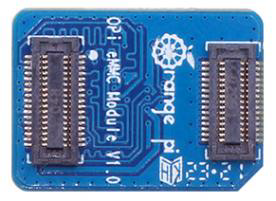
\includegraphics{img1/emmc2.png}
\item
  USB摄像头模块(可选) 可用于图像识别、视频通话等多方面用途。
  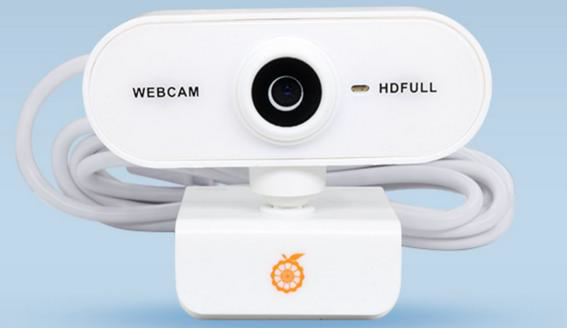
\includegraphics{img1/camera.png}
\item
  网线(可选)
  开发板自带有wifi模块可用于连接wifi,若需要更稳定的网络连接,建议使用网线连接。
  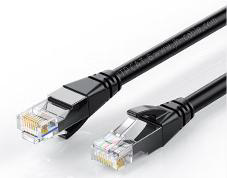
\includegraphics{img1/cable.png}
\item
  树莓派IMX219型号摄像头(MIPI-CSI)(可选)
  开发板带有两个MIPI-CSI接口,可以兼容树莓派的MIPI摄像头,无需占用USB接口。
  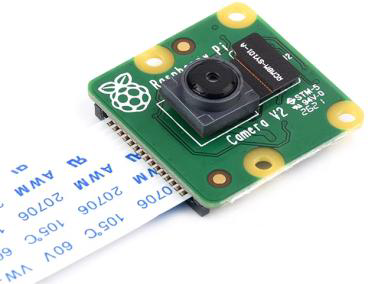
\includegraphics{img1/csi.png}
\item
  树莓派5寸MIPI LCD显示屏(可选)
  开发板带有一个MIPI-DSI显示输出接口,可以直接驱动MIPI的显示屏,而无需外接显示器。
  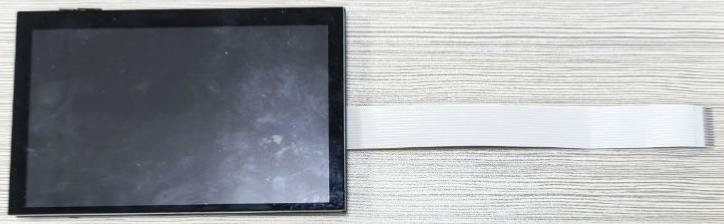
\includegraphics{img1/dsi.png}
\item
  Micro USB数据线(可选) 开发板自带了CH343P芯片,将UART转发为Micro
  USB接口,若需要使用串口对开发板进行调试,则需要使用Micro USB数据线。
  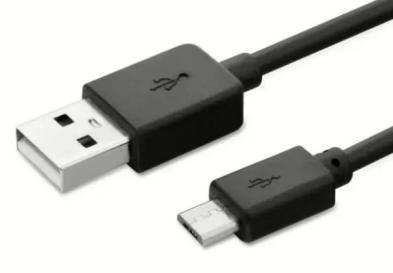
\includegraphics{img1/microusb.png}
\end{enumerate}

\hypertarget{ux4e0bux8f7dux5f00ux53d1ux677fux7684ux7cfbux7edfux955cux50cf}{%
\subsection{下载开发板的系统镜像}\label{ux4e0bux8f7dux5f00ux53d1ux677fux7684ux7cfbux7edfux955cux50cf}}

作为华为生态中重要的一员,开发板不仅支持Ubuntu系统,也支持openEuler系统,但由于开发板自身并无存储,我们在使用开发板的过程中需要使用电脑对TF卡进行系统的刷写,建议使用安装有Windows11
或 Ubuntu22.04以上版本的PC。

首先,打开香橙派官网的\href{http://www.orangepi.cn/html/hardWare/computerAndMicrocontrollers/service-and-support/Orange-Pi-AIpro.html}{技术支持界面}。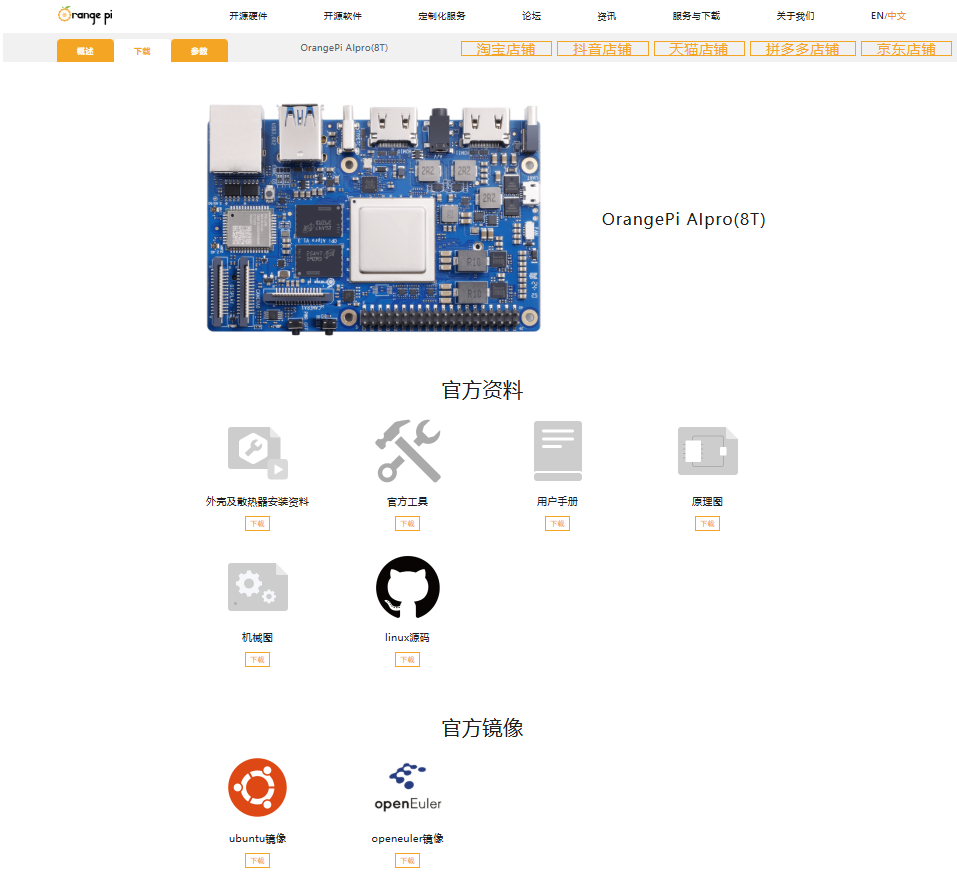
\includegraphics{img1/技术支持.png}

向下滑动网页,找到官方镜像部分,分为Ubuntu和openEuler两个部分,两个系统都是官方为我们编译完成的,且预装了部分昇腾NPU的应用环境以及软件,非常方便新手用户上手使用。

\includegraphics{img1/官方镜像.png}

\hypertarget{ubuntu}{%
\subsubsection{Ubuntu}\label{ubuntu}}

\begin{enumerate}
\def\labelenumi{\arabic{enumi}.}
\tightlist
\item
  点击下载
\includegraphics{img1/download_ubuntu.png}
\item
  复制提取码并跳转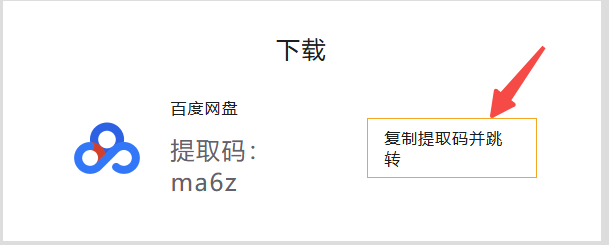
\includegraphics{img1/copyandjump.png}
\item
  打开百度网盘的链接后有一个命名为Ubuntu的文件夹,点开该文件夹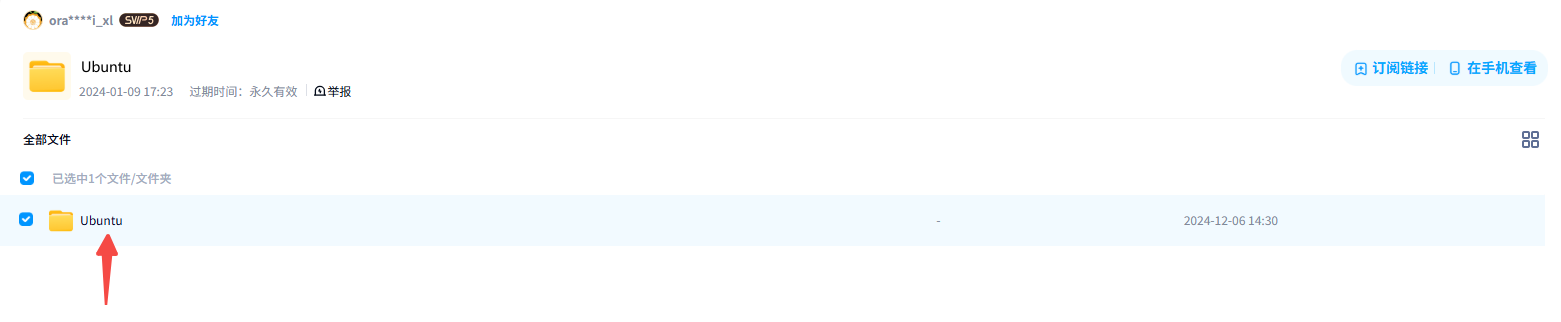
\includegraphics{img1/folder.png}
\item
  文件夹中,后缀为.xz的文件是镜像压缩包文件,.sha文件是压缩包的md5校验码文件,用于校验镜像包文件是否完整。
\item
  文件夹中的镜像有两种,一种文件名带有Desktop的,是带有GUI图形化界面的,另一种文件名带有minimal的,是不具有图形化界面的,只有命令行界面。建议新学习的用户使用带有desktop的镜像。
  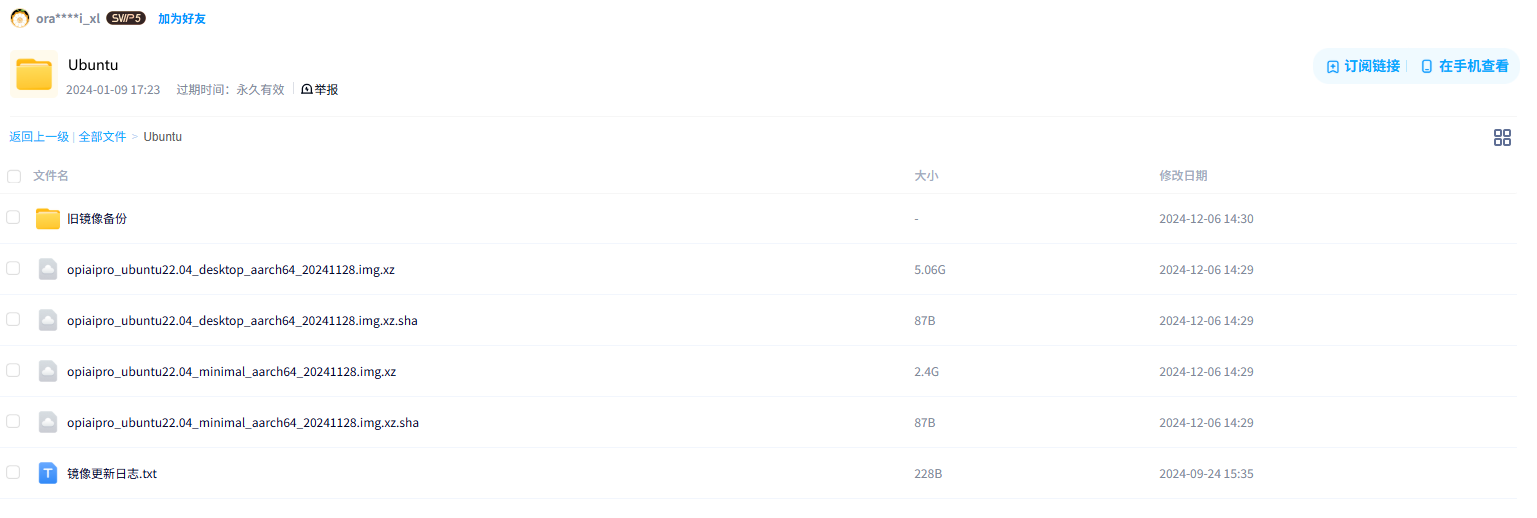
\includegraphics{img1/chooseubuntu.png}
\item
  下载后先校验压缩包是否完整,后解压压缩包
\end{enumerate}

\hypertarget{openeuler}{%
\subsubsection{openEuler}\label{openeuler}}

\begin{enumerate}
\def\labelenumi{\arabic{enumi}.}
\tightlist
\item
  点击下载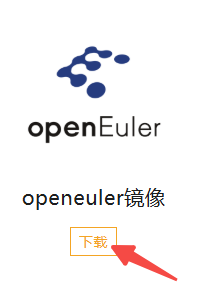
\includegraphics{img1/download_openeuler.png}
\item
  复制提取码并跳转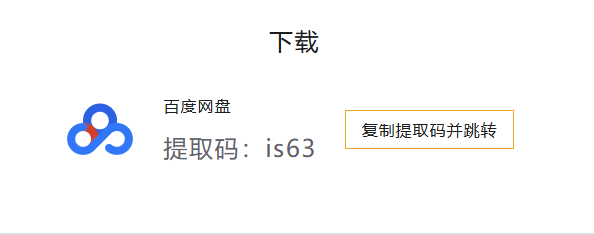
\includegraphics{img1/cpjp.png}
\item
  打开百度网盘的链接后有一个命名为OpenEuler的文件夹,点开该文件夹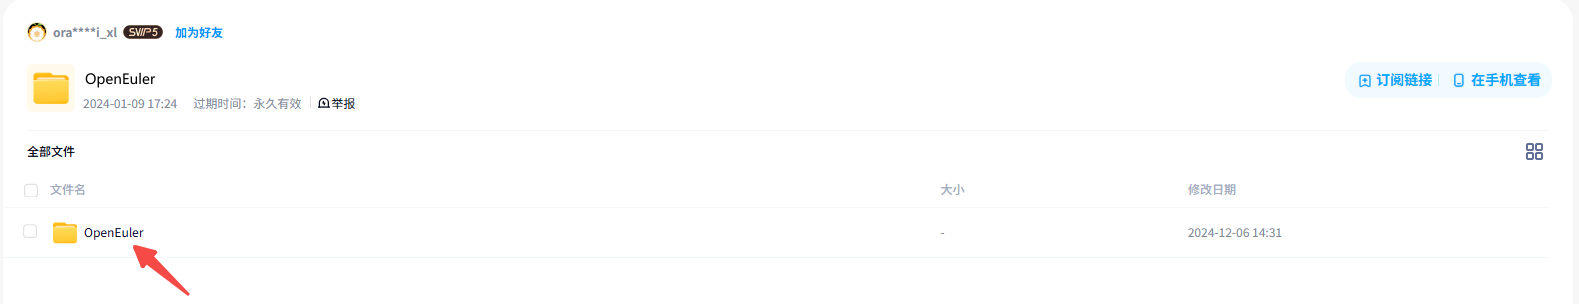
\includegraphics{img1/folderr.png}
\item
  文件夹中,后缀为.xz的文件是镜像压缩包文件,.sha文件是压缩包的md5校验码文件,用于校验镜像包文件是否完整。
\item
  文件夹中的镜像只有一种,即具有GUI图形化界面的openEuler系统。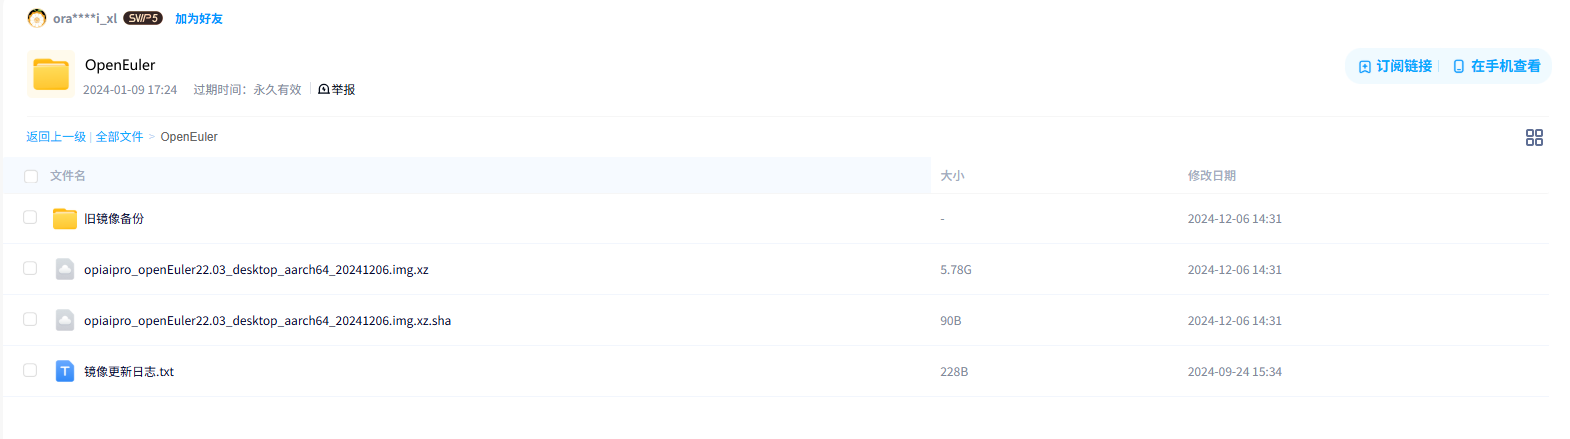
\includegraphics{img1/chooseeuler.png}
\item
  下载后先校验压缩包是否完整,后解压压缩包
\end{enumerate}

\hypertarget{ux4f7fux7528md5ux6821ux9a8cux4e0bux8f7dux7684ux6587ux4ef6}{%
\subsubsection{使用md5校验下载的文件}\label{ux4f7fux7528md5ux6821ux9a8cux4e0bux8f7dux7684ux6587ux4ef6}}

在Windows系统下,可以使用\texttt{certutil\ -hashfile\ \textless{}filename\textgreater{}\ md5};在Ubuntu系统下,可以使用\texttt{md5sum\ \textless{}filename\textgreater{}};在MacOS系统下,可以使用\texttt{md5\ \textless{}filename\textgreater{}}进行计算,此处以Windows系统为例:在文件夹按住Shift键并单击鼠标右键,选择``在终端(Powershell/命令提示符)中打开''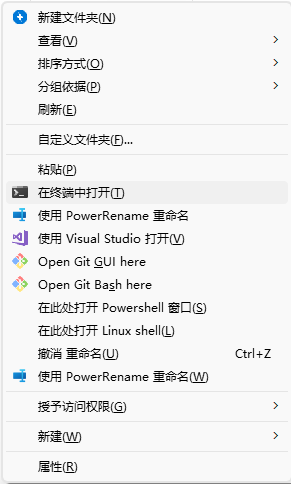
\includegraphics{img1/shell.png},然后在打开的窗口中输入\texttt{certutil\ -hashfile\ opiaipro\_ubuntu22.04\_desktop\_aarch64\_20241128.img.xz\ md5}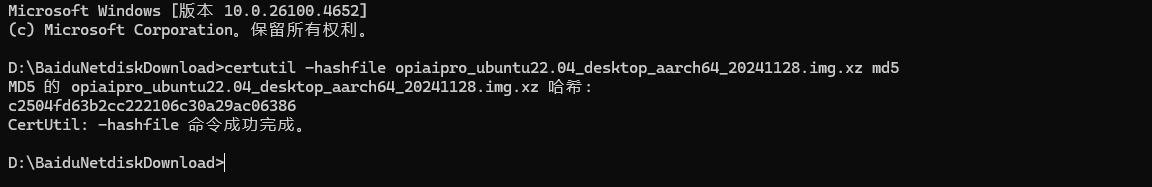
\includegraphics{img1/md5.png},将得到的md5值与\texttt{opiaipro\_ubuntu22.04\_desktop\_aarch64\_20241128.img.xz.sha}文件进行对比,若一致可进行下一步操作,否则需要重新下载。

\hypertarget{ux5237ux5199ux7cfbux7edfux5230tfux5361}{%
\subsection{刷写系统到TF卡}\label{ux5237ux5199ux7cfbux7edfux5230tfux5361}}

\hypertarget{ux4e0bux8f7dux5e76ux5b89ux88c5ux5fc5ux8981ux7684ux5de5ux5177}{%
\subsubsection{下载并安装必要的工具}\label{ux4e0bux8f7dux5e76ux5b89ux88c5ux5fc5ux8981ux7684ux5de5ux5177}}

\begin{quote}
下载链接:\href{http://www.orangepi.cn/html/hardWare/computerAndMicrocontrollers/service-and-support/Orange-Pi-AIpro.html}{官网}
\href{https://pan.baidu.com/s/1Jho73pw91r5GJD2KijY45Q?pwd=3xuz\#list/path=\%2F}{百度网盘}
1. SD Card Formatter
这个是TF卡的快速格式化工具,在每次需要刷写系统之前,都必须先对TF卡进行格式化操作,若不格式化在后续的刷写系统过程中有较大概率出错。
2. balenaEther 这个是系统镜像的刷写工具,用于刷写img镜像文件进入TF卡。
\end{quote}

\hypertarget{ux683cux5f0fux5316tfux5361}{%
\subsubsection{格式化TF卡}\label{ux683cux5f0fux5316tfux5361}}

\begin{enumerate}
\def\labelenumi{\arabic{enumi}.}
\tightlist
\item
  将TF卡插入读卡器中,并将读卡器插入电脑
\item
  打开SD Card Formatter软件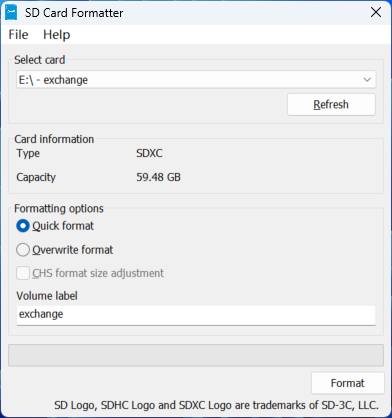
\includegraphics{img1/SDFmt.png}
\item
  点击右下角Format按键,格式化TF卡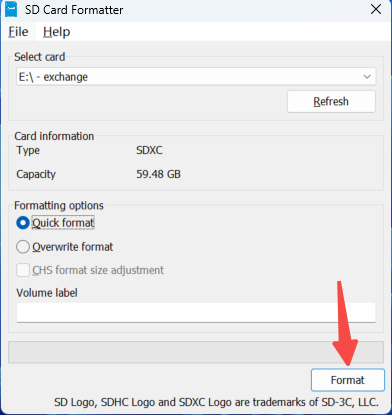
\includegraphics{img1/fmt.png}
  \textgreater{}
  警告内容是关于格式化操作会清除TF卡上原有的所有数据,此处选是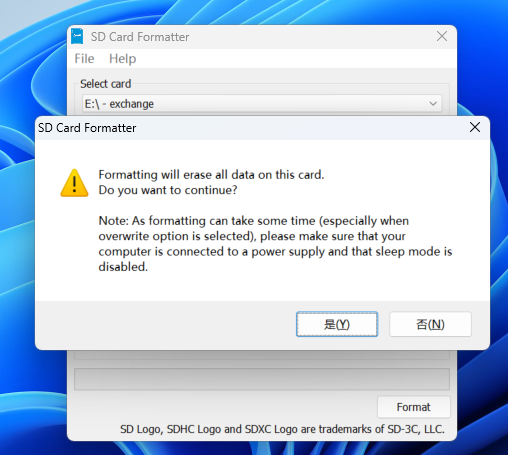
\includegraphics{img1/warning.png}
\item
  等待软件格式化完成,并点击确定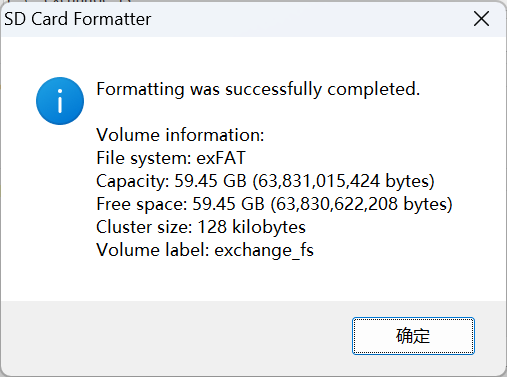
\includegraphics{img1/fmtfin.png}
\end{enumerate}

\hypertarget{ux5237ux5199ux7cfbux7edfux5230tfux5361ux4ee5ubuntuux4e3aux4f8b}{%
\subsubsection{刷写系统到TF卡(以Ubuntu为例)}\label{ux5237ux5199ux7cfbux7edfux5230tfux5361ux4ee5ubuntuux4e3aux4f8b}}

\begin{quote}
此处以Ubuntu为例 1.
打开balenaEther,选择``从文件烧录''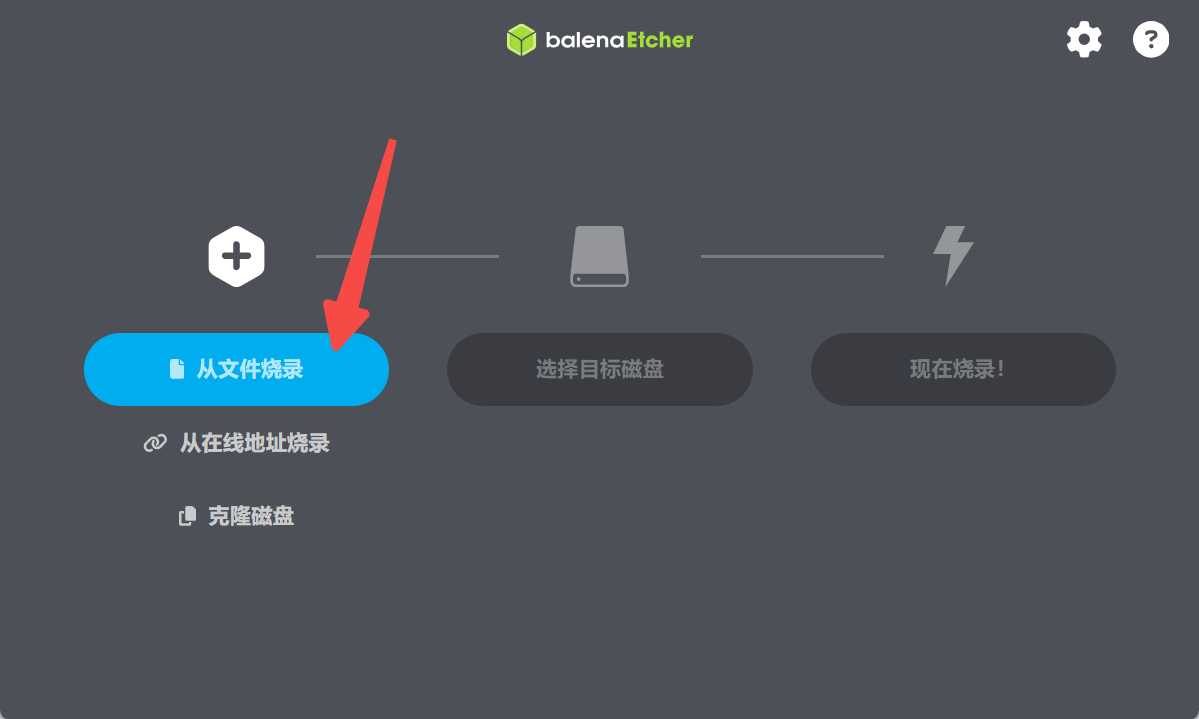
\includegraphics{img1/ether1.png} 2.
选择好要烧录的镜像文件(\textbf{.img}格式),再选择目标磁盘为TF卡对应的位置,如图中名称为``SDXC
Card''的位置,选中并选择``选定1''。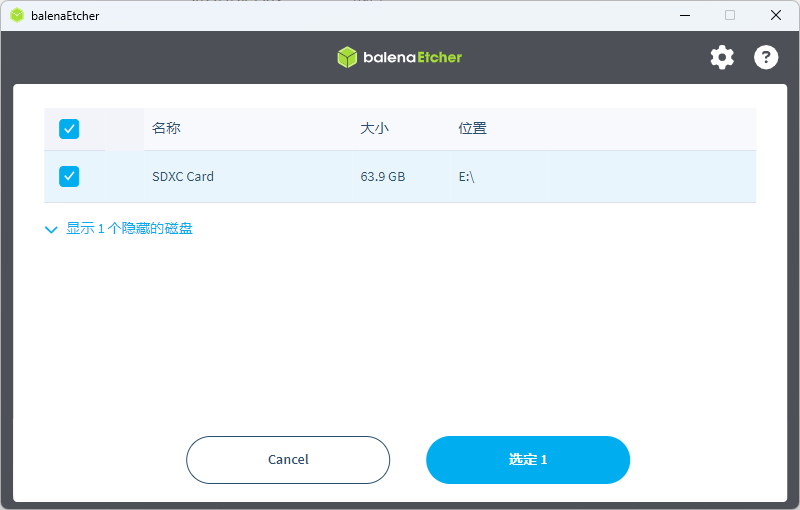
\includegraphics{img1/chooseether.png}
3. 点击``现在烧录!'',耐心等待烧录完成。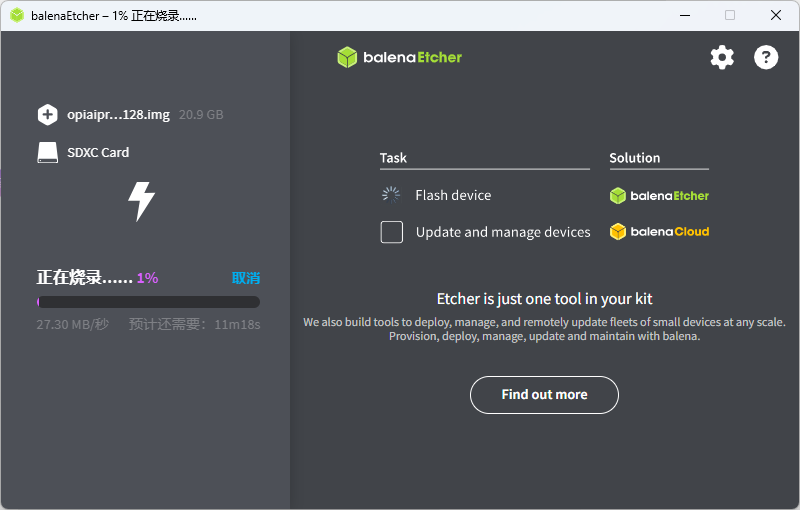
\includegraphics{img1/dd.png}
4. 烧录完成后进入校验过程,也请耐心等待。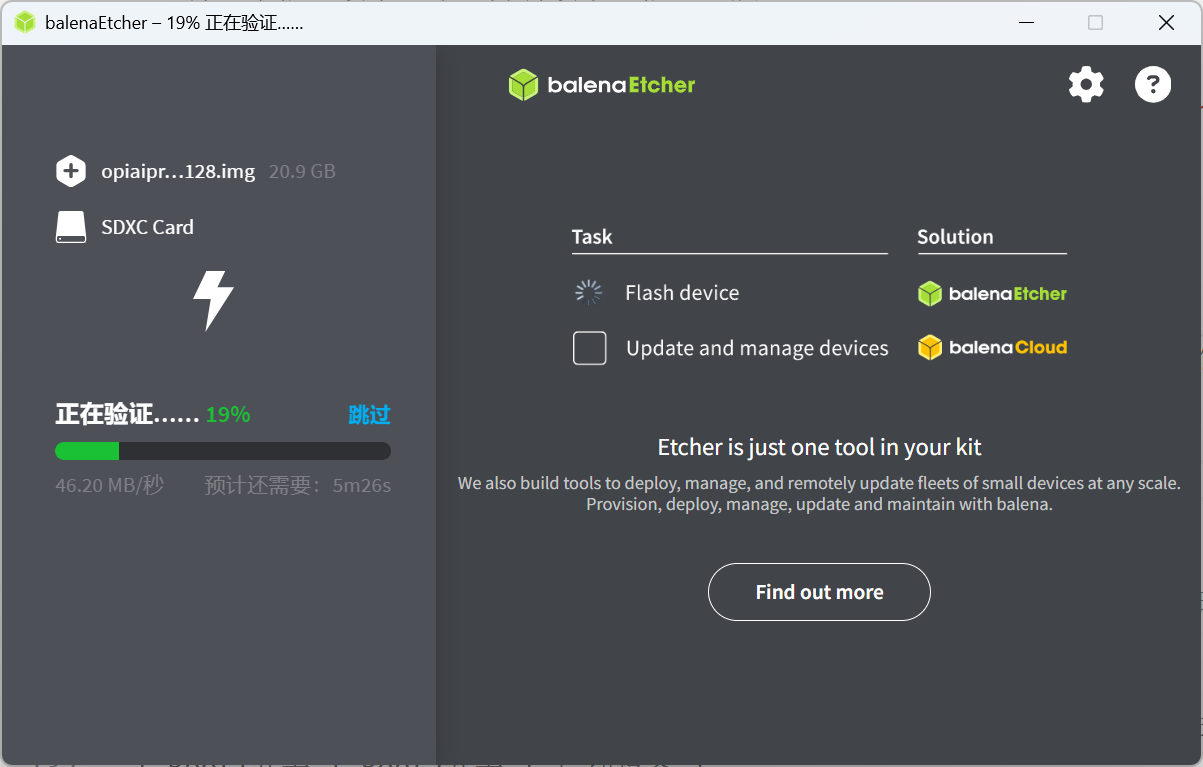
\includegraphics{img1/val.png}
5.
烧录完成后即可关闭程序,并安全弹出TF卡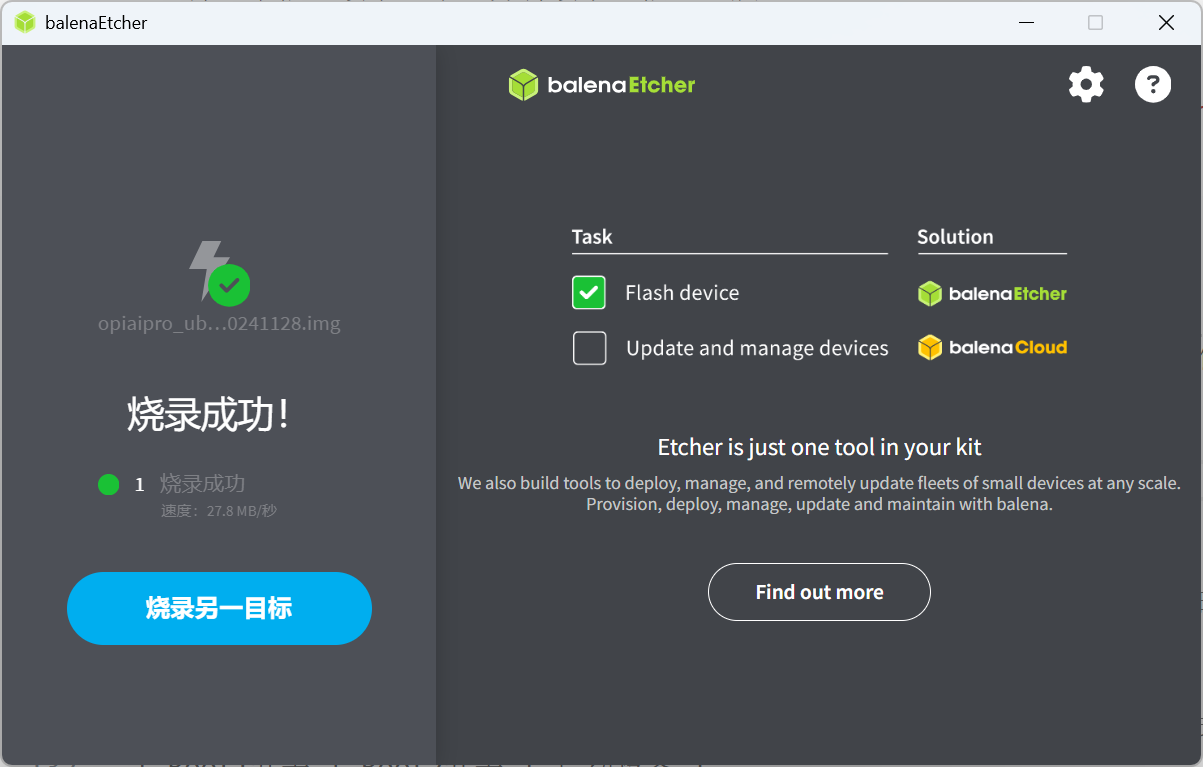
\includegraphics{img1/finish.png}
\end{quote}

\hypertarget{ux5237ux5199ux7cfbux7edfux5230emmc}{%
\subsubsection{刷写系统到eMMC}\label{ux5237ux5199ux7cfbux7edfux5230emmc}}

由于板上并不自带有eMMC模块,若要想使用需要额外购买香橙派的eMMC模块,此处暂时不列入参考,若需使用,请查阅香橙派的用户手册。

\hypertarget{ux5237ux5199ux7cfbux7edfux5230ssd}{%
\subsubsection{刷写系统到SSD}\label{ux5237ux5199ux7cfbux7edfux5230ssd}}

开发板带有M.2接口,可以使用SSD作为启动设备。但SSD需要自行准备,且根据香橙派

\hypertarget{ux8c03ux6574ux8bbeux5907ux542fux52a8ux65b9ux5f0fux7684ux62e8ux7801ux5f00ux5173}{%
\subsubsection{调整设备启动方式的拨码开关}\label{ux8c03ux6574ux8bbeux5907ux542fux52a8ux65b9ux5f0fux7684ux62e8ux7801ux5f00ux5173}}

开发板支持多种启动方式,包括TF卡、eMMC以及M.2
SSD,当这些存储设备都同时存在时,需要让开发板选定一个存储设备作为启动来源。
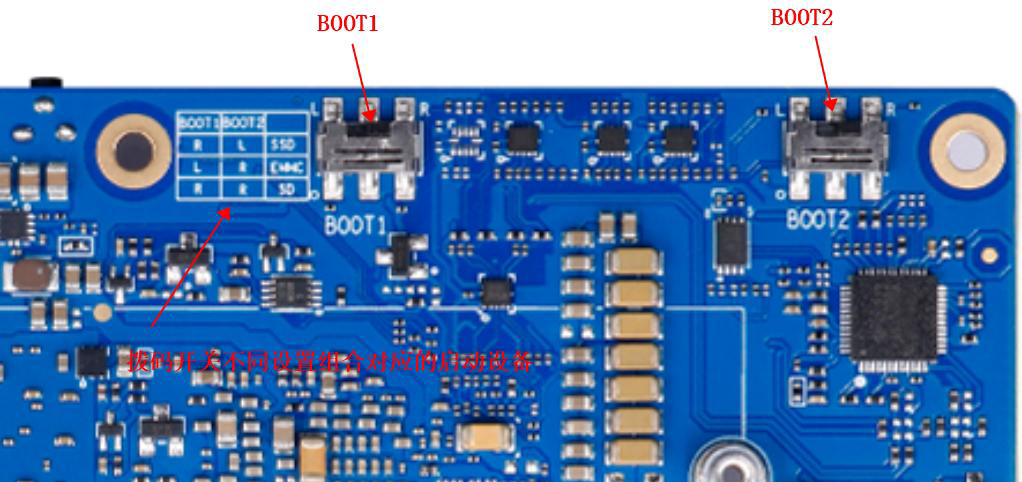
\includegraphics{img1/bootswitch.png}
两个开关都有左、右两种状态,因此共有4种状态,但是目前开发板仅使用3种模式,对应的参数表如下:
\textbar{} Boot1开关 \textbar{} Boot2开关 \textbar{} 启动设备 \textbar{}
\textbar{} :------: \textbar{} :------: \textbar{} :------: \textbar{}
\textbar{} 左 \textbar{} 左 \textbar{} 未使用 \textbar{} \textbar{} 右
\textbar{} 右 \textbar{} TF卡 \textbar{} \textbar{} 左 \textbar{} 右
\textbar{} eMMC \textbar{} \textbar{} 右 \textbar{} 左 \textbar{} M.2
SSD (Nvme或Ngff)\textbar{}
切换拨码开关后,必须要将开发板完全断电再重新上电才能使新的启动配置生效,使用RESET按键重启则不会使新的启动配置生效。

\hypertarget{ux542fux52a8ux5f00ux53d1ux677fubuntu}{%
\subsection{启动开发板(Ubuntu)}\label{ux542fux52a8ux5f00ux53d1ux677fubuntu}}

\begin{itemize}
\tightlist
\item
  图形化界面
\end{itemize}

\begin{enumerate}
\def\labelenumi{\arabic{enumi}.}
\tightlist
\item
  将系统刷写完成的TF卡从读卡器中取出,插入开发板的TF卡插槽中,并确保两个启动开关的位置均在右边,接入HDMI数据线到靠近USB3.0接口的HDMI0接口,然后将Type-C电源线插入开发板最边缘的TYPE-C供电口,等待风扇的声音变小以及屏幕出现系统登录界面。
  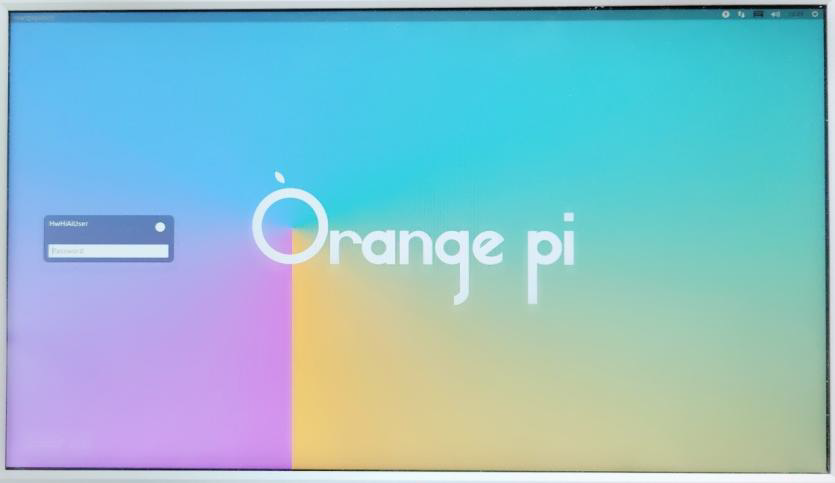
\includegraphics{img1/beforelogin.png}
\item
  进入登录界面后,将键盘接入开发板的USB接口中,默认的登录用户名是\texttt{HwHiAiUser},输入该账户的密码\texttt{Mind@123},登录进入系统。
  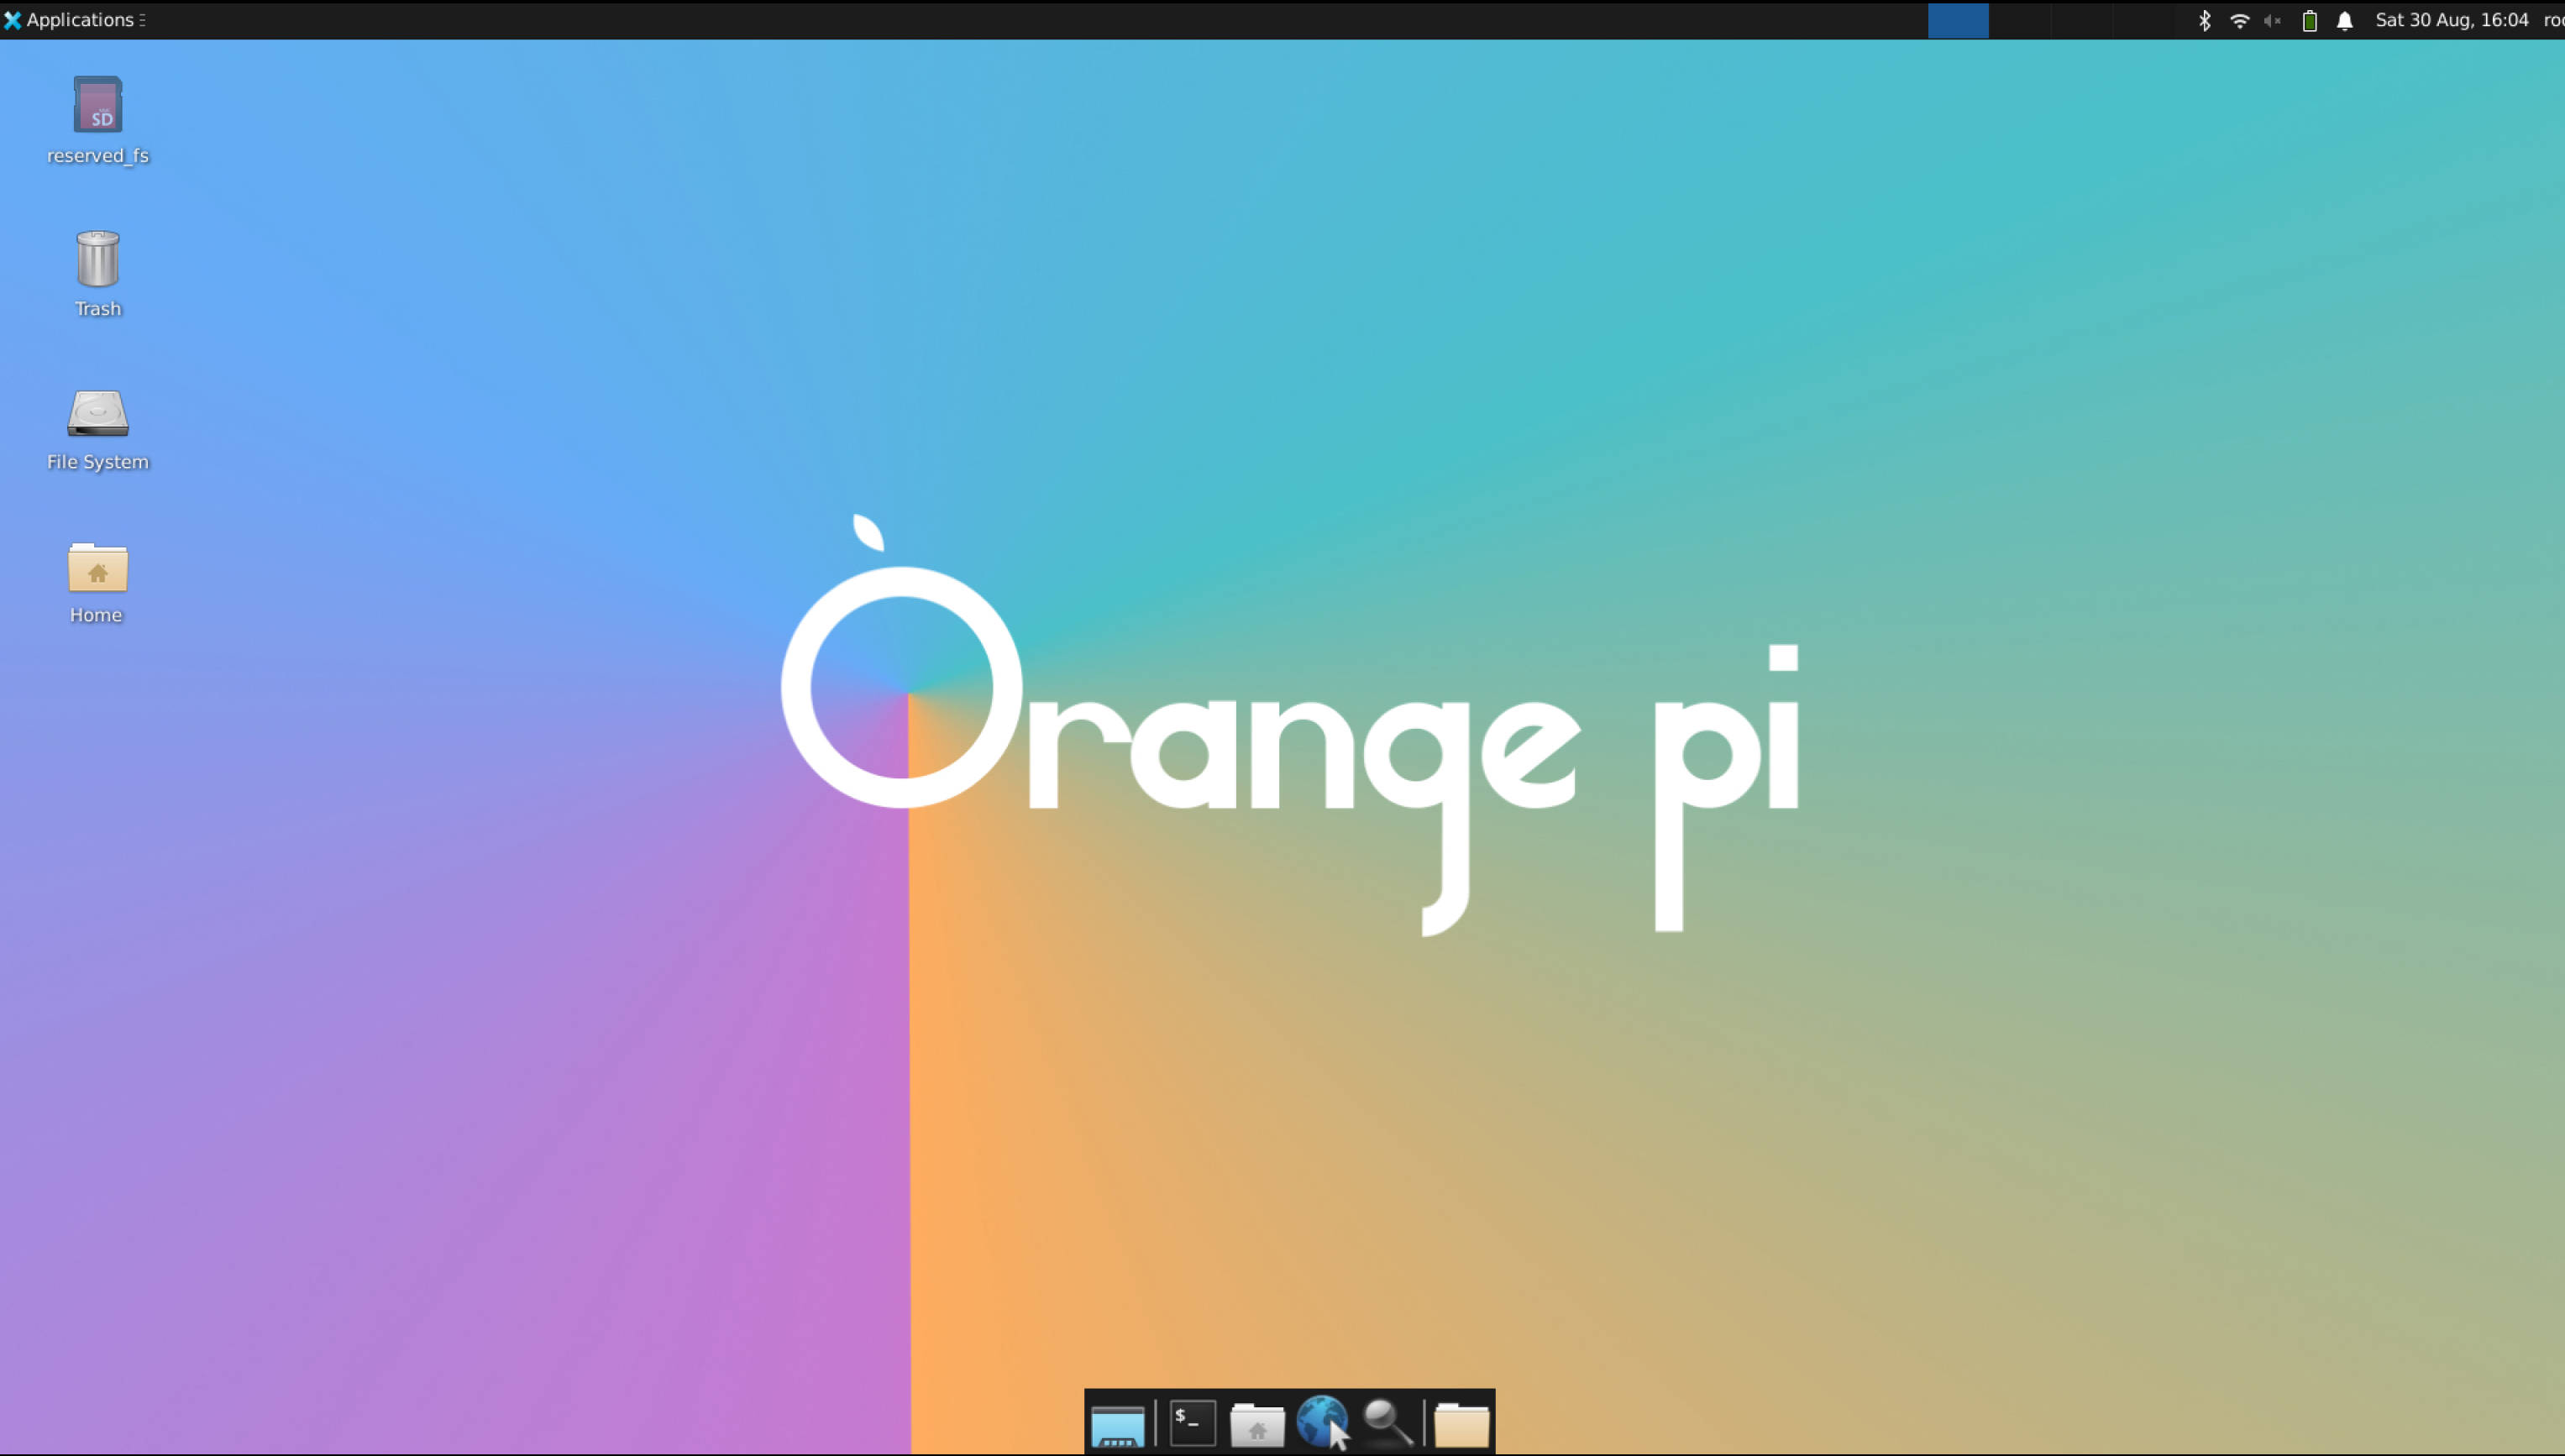
\includegraphics{img1/logingui.png} 默认账户表格: \textbar{} 用户名
  \textbar{} 密码 \textbar{} \textbar{} :---: \textbar{} :--: \textbar{}
  \textbar{} root \textbar{} Mind@123 \textbar{} \textbar{} HwHiAiUser
  \textbar{} Mind@123 \textbar{}
\end{enumerate}

\begin{itemize}
\tightlist
\item
  串口界面
\end{itemize}

\begin{enumerate}
\def\labelenumi{\arabic{enumi}.}
\tightlist
\item
  使用USB2TTL模块,与开发板的GPIO口进行连线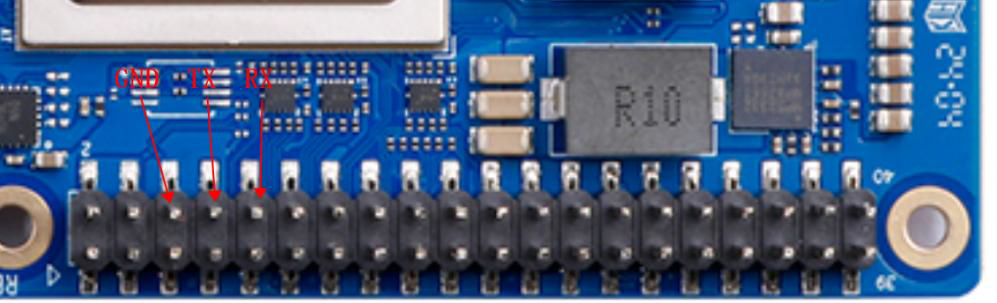
\includegraphics{img1/gpio_ttl.png},开发板的TX(GPIO8)接入USB2TTL模块的RX接口,开发板的RX(GPIO10)则接入模块的TX接口,并连接好GND接地,在Windows电脑下可以使用PUTTY连接串口。
\item
  使用开发板自带的Micro
  USB接口进行串口调试,该方法更为方便,只需要一根Micro
  USB数据线,接入电脑后打开设备管理器查询对应的串口,然后使用PUTTY进行链接即可。
  以Micro USB接口为例:
\item
  使用Micro USB数据线连接开发板和电脑
\item
  打开电脑的设备管理器,选择端口,寻找开发板对应的串口端口号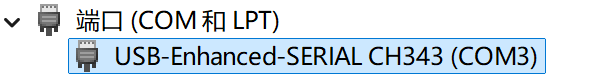
\includegraphics{img1/ttl.png}
\item
  打开串口调试软件(PUTTY)\includegraphics{img1/putty.png},将Connection
  Type选择为\texttt{Serial},然后在Serial
  Line处将端口号修改为设备管理器中查到的端口号,如作者此处端口号为\texttt{COM3},此外,还需要将Speed从9600修改为115200,最后点击Open打开串口。
\item
  等待出现\texttt{Ubuntu\ 22.04.3\ LTS\ orangepiaipro\ ttyAM0}字样,输入登录的用户名HwHiAiUser并回车,然后输入密码Mind@123并回车,注意在输入密码的时候屏幕并不会显示任何东西,登陆后的界面如图所示。
  \includegraphics{img1/serial.png} \includegraphics{img1/login.png}
\end{enumerate}

\hypertarget{ubuntu-xfceux684cux9762ux4f7fux7528ux8bf4ux660e}{%
\subsection{Ubuntu
Xfce桌面使用说明}\label{ubuntu-xfceux684cux9762ux4f7fux7528ux8bf4ux660e}}

目前系统仅支持Ubuntu 22.04 - Jammy系统,内核版本为Linux 5.10 \#\#\#\#
当前版本适配情况
请详见香橙派官方的用户手册,有部分功能仅支持使用官方程序进行测试,无法直接从系统中调用,在使用过程中需注意这些限制。

\hypertarget{hdmiux53e3ux4f7fux7528}{%
\subsubsection{HDMI口使用}\label{hdmiux53e3ux4f7fux7528}}

开发板有两个HDMI2.0 接口,目前只有HDMI0 支持显示Linux
系统的桌面,当Linux 系统的桌面系统关闭时,HDMI0 和HDMI1 还可以用于NVR
二次开 发场景输出图片。

\hypertarget{ux97f3ux9891ux4f7fux7528}{%
\subsubsection{音频使用}\label{ux97f3ux9891ux4f7fux7528}}

Linux 内核没有适配耳机和HDMI 等的ALSA 音频驱动,此部分驱动还在开
发中,目前只能通过音频样例代码来测试耳机、HDMI 的音频播放和板载MIC
的录音功能。或者自行购买Linux系统免驱的USB外置声卡,经测试可以正常使用。


\backmatter
\chapter*{致谢}
感谢关注与贡献者。

\end{document}
